\documentclass[11pt]{article}

\usepackage[T1]{fontenc}
\usepackage{lmodern}
\usepackage{amsmath,amssymb,amsthm,mathtools}
\usepackage[margin=1in]{geometry}
\usepackage{microtype}
\usepackage{needspace}
\usepackage{tikz}
\usetikzlibrary{arrows.meta,decorations.markings}
\usepackage{mathtools}
\mathtoolsset{showonlyrefs}
\usepackage[font=small,labelfont=bf]{caption}
\usepackage[hidelinks]{hyperref}
\hypersetup{
  pdftitle={A noncircular oval with convex unit-tangent iterates},
  pdfauthor={Dean Menezes}
}
\allowdisplaybreaks[1]
\numberwithin{equation}{section}
\newtheorem{theorem}{Theorem}[section]
\newtheorem{proposition}[theorem]{Proposition}
\newtheorem{lemma}[theorem]{Lemma}
\newcommand{\R}{{\bf R}}
\newcommand{\Z}{{\bf Z}}
\newcommand{\Tmap}{\mathcal T}
\newcommand{\Bmap}{\mathcal B}
\newcommand{\eps}{\varepsilon}
\newcommand{\abs}[1]{\lvert #1\rvert}
\newcommand{\norm}[1]{\lVert #1\rVert}
\DeclareMathOperator{\Per}{Per}

\title{A noncircular oval with convex unit-tangent iterates}
\author{Dean Menezes}
\date{}

\begin{document}
\maketitle

\begin{abstract}
For an oriented regular plane curve \(\gamma\), define
\(\Tmap\gamma=\gamma+\tau\), where \(\tau\) is the positive unit tangent.
We prove that there is a smooth noncircular strictly convex closed curve
\(\Gamma\) such that \(\Tmap^n\Gamma\) is smooth and strictly convex for
every \(n\geq0\), answering a question of Tabachnikov. The proof starts
with a complete convex hairpin $C$ such that $\Tmap C$ is a translated copy of $C$.
Periodizing its steering profile gives long closed convex models forming an
approximate backward orbit with exponentially small \(L^1\) curvature
error. A regularizing inverse estimate shadows this approximate orbit by an
exact infinite orbit. The initial curve is close to a long model of bounded
width, so it cannot be a circle.
\end{abstract}

\section{Introduction}

The unit-tangent transform sends a circle of radius \(r\) to a circle of
radius \(\sqrt{r^2+1}\). We show that a noncircular oval can also remain
convex under every iterate.

Let \(\gamma:\R/L\Z\to\R^2\) be a smooth regular closed curve,
parametrized by arclength, and let \(\tau_\gamma=\gamma'\) be its unit tangent.
The \emph{unit-tangent transform} is the oriented curve
\begin{equation}\label{eq:Tdef}
  \Tmap\gamma=\gamma+\tau_\gamma.
\end{equation}
Curves are identified under orientation-preserving regular
reparametrization, so \(\Tmap\) is independent of parametrization. Before
each iterate, we reparametrize by arclength. Convex curves are
oriented counterclockwise, with inward unit normal \(\nu\) and
\(\tau'=k\nu\). A convex closed curve is the boundary of a convex body,
traversed once. An \emph{oval} is a smooth convex closed curve with
\(k>0\) everywhere.

Tabachnikov asked whether an oval all of whose unit-tangent iterates are
convex must be a circle \cite[Section~9]{Tabachnikov2015},
\cite[Conjecture~4]{Tabachnikov2023}. We answer this question in the negative:

\begin{theorem}\label{thm:main}
There is a noncircular oval \(\Gamma_0\) such that \(\Tmap^n\Gamma_0\) is an
oval for every integer \(n\geq0\).
\end{theorem}

The construction uses long ovals of bounded transverse width. Their local
model is a complete convex hairpin that \(\Tmap\) carries to a horizontal
translate; see Figure~\ref{fig:models}.

In the bicycle model, \(R\) and \(F=\Tmap R\) are the rear and front
tracks of a unit segment. The steering equation describes the angle
between their tangents \cite[Section~2]{LeviTabachnikov}; see also
\cite[Proposition~2.6]{BorLeviPerlineTabachnikov2020}. For a convex closed
front of curvature less than one, this equation selects a unique convex rear
on the branch where the steering angle lies between \(0\) and \(\pi/2\).
We denote this inverse by \(\Bmap\).

Sections~\ref{sec:translator}--\ref{sec:matching} construct exact closed
pairs \(\Tmap R_H=F_H\) and show that \(R_H\) and \(F_{P(H)}\) have
exponentially close intrinsic curvatures, where
\(P(H)=H-\Delta+o(1)\) and \(\Delta>0\). Section~\ref{sec:shadow} turns
these approximate inverse steps into an exact orbit. Section~\ref{sec:application}
excludes a circle by comparing width and perimeter.

\begin{figure}[tb]
\centering
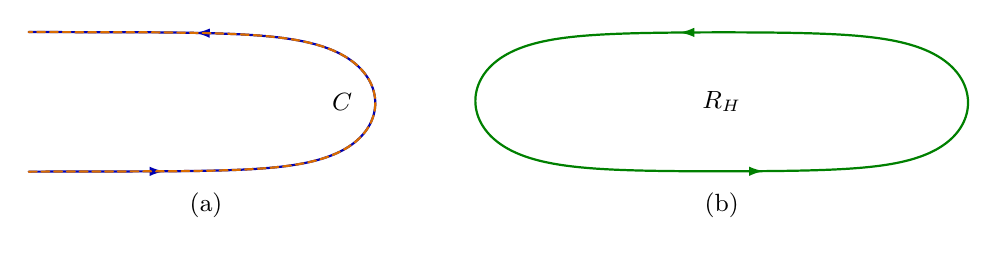
\begin{tikzpicture}[
  x=1cm,y=1cm,
  line cap=round,line join=round,
  model/.style={line width=.8pt,draw=blue!70!black},
  front/.style={line width=.8pt,draw=orange!85!black,dash pattern=on 2.8pt off 1.8pt},
  oval/.style={line width=.8pt,draw=green!50!black},
  orient/.style={postaction={decorate},decoration={markings,
    mark=at position .18 with {\arrow{Latex[length=1.9mm,width=1.2mm]}},
    mark=at position .78 with {\arrow{Latex[length=1.9mm,width=1.2mm]}}}},
  closedorient/.style={postaction={decorate},decoration={markings,
    mark=at position .04 with {\arrow{Latex[length=1.9mm,width=1.2mm]}},
    mark=at position .54 with {\arrow{Latex[length=1.9mm,width=1.2mm]}}}},
  every node/.style={font=\small}
]
% Numerical coordinates are embedded; no external drawing data are needed.
% Piecewise-linear rendering avoids spurious spline inflections.
\draw[model,orient] plot coordinates {
(0.70000000,-0.88671512) (2.45288413,-0.88239658) (2.82262401,-0.87807804) (3.04172361,-0.87375948) (3.19796068,-0.86944089)
(3.31946722,-0.86512228) (3.41890044,-0.86080363) (3.50305197,-0.85648495) (3.57599172,-0.85216621) (3.64035225,-0.84784741)
(3.69793486,-0.84352855) (3.75002645,-0.83920963) (3.79757851,-0.83489062) (3.84131438,-0.83057153) (3.88179684,-0.82625235)
(3.91947238,-0.82193307) (3.95470117,-0.81761369) (3.98777798,-0.81329419) (4.01894711,-0.80897458) (4.04841329,-0.80465483)
(4.07634979,-0.80033496) (4.10290457,-0.79601494) (4.12820493,-0.79169478) (4.15236127,-0.78737447) (4.17546986,-0.78305399)
(4.19761523,-0.77873335) (4.21887196,-0.77441253) (4.23930619,-0.77009153) (4.25897687,-0.76577035) (4.27793673,-0.76144897)
(4.29623316,-0.75712738) (4.31390887,-0.75280559) (4.33100253,-0.74848358) (4.34754923,-0.74416135) (4.36358091,-0.73983889)
(4.37912675,-0.73551620) (4.39421346,-0.73119326) (4.40886556,-0.72687008) (4.42310559,-0.72254663) (4.43695435,-0.71822293)
(4.45043107,-0.71389895) (4.46355353,-0.70957470) (4.47633824,-0.70525017) (4.48880054,-0.70092535) (4.50095471,-0.69660023)
(4.51281408,-0.69227480) (4.52439108,-0.68794907) (4.53569736,-0.68362303) (4.54674380,-0.67929666) (4.55754064,-0.67496996)
(4.56809748,-0.67064292) (4.57842336,-0.66631555) (4.58852677,-0.66198782) (4.59841575,-0.65765974) (4.60809786,-0.65333130)
(4.61758024,-0.64900249) (4.62686967,-0.64467331) (4.63597254,-0.64034375) (4.64489492,-0.63601380) (4.65364257,-0.63168345)
(4.66222094,-0.62735271) (4.67063524,-0.62302156) (4.67889039,-0.61869000) (4.68699110,-0.61435802) (4.69494184,-0.61002561)
(4.70274688,-0.60569278) (4.71041028,-0.60135950) (4.71793593,-0.59702579) (4.72532753,-0.59269162) (4.73258864,-0.58835701)
(4.73972265,-0.58402192) (4.74673279,-0.57968638) (4.75362219,-0.57535035) (4.76039381,-0.57101385) (4.76705051,-0.56667687)
(4.77359504,-0.56233939) (4.78003001,-0.55800142) (4.78635795,-0.55366294) (4.79258129,-0.54932395) (4.79870236,-0.54498445)
(4.80472339,-0.54064443) (4.81064655,-0.53630388) (4.81647390,-0.53196281) (4.82220745,-0.52762119) (4.82784912,-0.52327903)
(4.83340076,-0.51893632) (4.83886417,-0.51459306) (4.84424106,-0.51024924) (4.84953310,-0.50590486) (4.85474190,-0.50155990)
(4.85986901,-0.49721437) (4.86491592,-0.49286825) (4.86988407,-0.48852155) (4.87477488,-0.48417426) (4.87958968,-0.47982636)
(4.88432979,-0.47547787) (4.88899647,-0.47112877) (4.89359095,-0.46677905) (4.89811439,-0.46242872) (4.90256796,-0.45807776)
(4.90695277,-0.45372618) (4.91126988,-0.44937396) (4.91552033,-0.44502110) (4.91970515,-0.44066760) (4.92382530,-0.43631345)
(4.92788173,-0.43195865) (4.93187537,-0.42760319) (4.93580711,-0.42324706) (4.93967780,-0.41889027) (4.94348829,-0.41453281)
(4.94723940,-0.41017467) (4.95093192,-0.40581584) (4.95456660,-0.40145633) (4.95814421,-0.39709613) (4.96166545,-0.39273524)
(4.96513105,-0.38837364) (4.96854166,-0.38401134) (4.97189797,-0.37964833) (4.97520062,-0.37528461) (4.97845022,-0.37092017)
(4.98164740,-0.36655500) (4.98479274,-0.36218912) (4.98788681,-0.35782250) (4.99093017,-0.35345515) (4.99392338,-0.34908706)
(4.99686695,-0.34471822) (4.99976140,-0.34034864) (5.00260723,-0.33597831) (5.00540492,-0.33160723) (5.00815495,-0.32723539)
(5.01085778,-0.32286278) (5.01351384,-0.31848941) (5.01612359,-0.31411527) (5.01868743,-0.30974036) (5.02120577,-0.30536467)
(5.02367903,-0.30098820) (5.02610758,-0.29661094) (5.02849181,-0.29223290) (5.03083207,-0.28785407) (5.03312874,-0.28347444)
(5.03538214,-0.27909402) (5.03759263,-0.27471279) (5.03976053,-0.27033076) (5.04188616,-0.26594793) (5.04396982,-0.26156428)
(5.04601182,-0.25717982) (5.04801245,-0.25279454) (5.04997200,-0.24840844) (5.05189073,-0.24402152) (5.05376892,-0.23963378)
(5.05560684,-0.23524520) (5.05740472,-0.23085580) (5.05916281,-0.22646556) (5.06088136,-0.22207448) (5.06256059,-0.21768256)
(5.06420072,-0.21328981) (5.06580198,-0.20889620) (5.06736457,-0.20450175) (5.06888869,-0.20010646) (5.07037455,-0.19571030)
(5.07182232,-0.19131330) (5.07323220,-0.18691544) (5.07460436,-0.18251672) (5.07593898,-0.17811714) (5.07723621,-0.17371669)
(5.07849622,-0.16931538) (5.07971917,-0.16491320) (5.08090520,-0.16051016) (5.08205445,-0.15610624) (5.08316706,-0.15170145)
(5.08424316,-0.14729578) (5.08528289,-0.14288924) (5.08628635,-0.13848182) (5.08725367,-0.13407352) (5.08818496,-0.12966434)
(5.08908033,-0.12525427) (5.08993986,-0.12084332) (5.09076367,-0.11643149) (5.09155184,-0.11201877) (5.09230445,-0.10760515)
(5.09302160,-0.10319065) (5.09370334,-0.09877526) (5.09434977,-0.09435897) (5.09496094,-0.08994179) (5.09553692,-0.08552372)
(5.09607776,-0.08110475) (5.09658352,-0.07668488) (5.09705425,-0.07226412) (5.09748999,-0.06784245) (5.09789078,-0.06341989)
(5.09825666,-0.05899643) (5.09858766,-0.05457207) (5.09888380,-0.05014681) (5.09914511,-0.04572064) (5.09937161,-0.04129357)
(5.09956331,-0.03686560) (5.09972022,-0.03243673) (5.09984235,-0.02800695) (5.09992969,-0.02357627) (5.09998224,-0.01914469)
(5.10000000,-0.01471220) (5.09998295,-0.01027881) (5.09993108,-0.00584451) (5.09984436,-0.00140931) (5.09972277,0.00302680)
(5.09956629,0.00746381) (5.09937487,0.01190172) (5.09914849,0.01634054) (5.09888709,0.02078026) (5.09859063,0.02522088)
(5.09825907,0.02966241) (5.09789234,0.03410484) (5.09749038,0.03854817) (5.09705314,0.04299241) (5.09658054,0.04743754)
(5.09607251,0.05188358) (5.09552897,0.05633051) (5.09494984,0.06077834) (5.09433503,0.06522707) (5.09368445,0.06967670)
(5.09299801,0.07412722) (5.09227561,0.07857864) (5.09151713,0.08303095) (5.09072247,0.08748415) (5.08989151,0.09193825)
(5.08902414,0.09639324) (5.08812022,0.10084911) (5.08717963,0.10530588) (5.08620223,0.10976353) (5.08518788,0.11422206)
(5.08413643,0.11868148) (5.08304774,0.12314178) (5.08192165,0.12760296) (5.08075799,0.13206502) (5.07955660,0.13652796)
(5.07831730,0.14099177) (5.07703992,0.14545646) (5.07572427,0.14992201) (5.07437016,0.15438844) (5.07297740,0.15885573)
(5.07154578,0.16332389) (5.07007508,0.16779292) (5.06856511,0.17226280) (5.06701563,0.17673354) (5.06542642,0.18120514)
(5.06379723,0.18567760) (5.06212784,0.19015091) (5.06041799,0.19462506) (5.05866743,0.19910007) (5.05687588,0.20357592)
(5.05504309,0.20805261) (5.05316877,0.21253014) (5.05125263,0.21700851) (5.04929439,0.22148771) (5.04729374,0.22596775)
(5.04525038,0.23044861) (5.04316397,0.23493030) (5.04103420,0.23941281) (5.03886072,0.24389614) (5.03664320,0.24838029)
(5.03438128,0.25286525) (5.03207459,0.25735102) (5.02972276,0.26183760) (5.02732540,0.26632498) (5.02488213,0.27081317)
(5.02239253,0.27530215) (5.01985620,0.27979192) (5.01727269,0.28428249) (5.01464159,0.28877384) (5.01196242,0.29326598)
(5.00923474,0.29775890) (5.00645806,0.30225259) (5.00363191,0.30674705) (5.00075577,0.31124229) (4.99782914,0.31573829)
(4.99485148,0.32023505) (4.99182226,0.32473257) (4.98874091,0.32923084) (4.98560686,0.33372986) (4.98241953,0.33822963)
(4.97917831,0.34273013) (4.97588257,0.34723138) (4.97253168,0.35173336) (4.96912499,0.35623606) (4.96566181,0.36073950)
(4.96214145,0.36524365) (4.95856320,0.36974852) (4.95492632,0.37425410) (4.95123006,0.37876038) (4.94747365,0.38326737)
(4.94365627,0.38777506) (4.93977711,0.39228344) (4.93583532,0.39679251) (4.93183002,0.40130226) (4.92776033,0.40581270)
(4.92362531,0.41032380) (4.91942401,0.41483558) (4.91515544,0.41934803) (4.91081860,0.42386113) (4.90641245,0.42837489)
(4.90193589,0.43288930) (4.89738784,0.43740435) (4.89276713,0.44192005) (4.88807259,0.44643638) (4.88330299,0.45095334)
(4.87845709,0.45547092) (4.87353357,0.45998913) (4.86853110,0.46450795) (4.86344828,0.46902738) (4.85828369,0.47354741)
(4.85303583,0.47806804) (4.84770317,0.48258927) (4.84228412,0.48711108) (4.83677705,0.49163348) (4.83118024,0.49615645)
(4.82549193,0.50067999) (4.81971030,0.50520410) (4.81383345,0.50972877) (4.80785943,0.51425399) (4.80178618,0.51877976)
(4.79561160,0.52330608) (4.78933350,0.52783293) (4.78294959,0.53236032) (4.77645751,0.53688823) (4.76985478,0.54141666)
(4.76313885,0.54594560) (4.75630706,0.55047505) (4.74935662,0.55500500) (4.74228464,0.55953545) (4.73508812,0.56406639)
(4.72776389,0.56859782) (4.72030869,0.57312972) (4.71271909,0.57766209) (4.70499150,0.58219493) (4.69712220,0.58672823)
(4.68910726,0.59126198) (4.68094258,0.59579618) (4.67262389,0.60033082) (4.66414668,0.60486589) (4.65550622,0.60940139)
(4.64669758,0.61393732) (4.63771555,0.61847366) (4.62855465,0.62301041) (4.61920913,0.62754756) (4.60967293,0.63208511)
(4.59993965,0.63662304) (4.59000256,0.64116136) (4.57985451,0.64570006) (4.56948800,0.65023913) (4.55889504,0.65477856)
(4.54806720,0.65931835) (4.53699551,0.66385849) (4.52567046,0.66839897) (4.51408196,0.67293979) (4.50221922,0.67748094)
(4.49007078,0.68202242) (4.47762439,0.68656421) (4.46486696,0.69110631) (4.45178447,0.69564872) (4.43836189,0.70019142)
(4.42458309,0.70473441) (4.41043069,0.70927769) (4.39588598,0.71382124) (4.38092875,0.71836506) (4.36553711,0.72290914)
(4.34968735,0.72745348) (4.33335368,0.73199807) (4.31650801,0.73654290) (4.29911968,0.74108797) (4.28115507,0.74563326)
(4.26257731,0.75017877) (4.24334574,0.75472450) (4.22341545,0.75927044) (4.20273664,0.76381658) (4.18125387,0.76836290)
(4.15890522,0.77290942) (4.13562115,0.77745611) (4.11132331,0.78200298) (4.08592291,0.78655001) (4.05931878,0.79109720)
(4.03139500,0.79564454) (4.00201785,0.80019202) (3.97103198,0.80473964) (3.93825548,0.80928739) (3.90347345,0.81383526)
(3.86642952,0.81838325) (3.82681444,0.82293134) (3.78425041,0.82747954) (3.73826929,0.83202783) (3.68828118,0.83657621)
(3.63352823,0.84112466) (3.57301410,0.84567319) (3.50539202,0.85022178) (3.42877841,0.85477043) (3.34042319,0.85931914)
(3.23608036,0.86386788) (3.10867753,0.86841666) (2.94507054,0.87296547) (2.71618165,0.87751431) (2.33221252,0.88206315)
(0.70000000,0.88661201)
};
\draw[front] plot coordinates {
(0.70000000,-0.88671527) (2.47399116,-0.88222400) (2.84416535,-0.87773273) (3.06341103,-0.87324147) (3.21971884,-0.86875022)
(3.34126481,-0.86425899) (3.44072102,-0.85976777) (3.52488553,-0.85527658) (3.59783148,-0.85078541) (3.66219322,-0.84629427)
(3.71977315,-0.84180317) (3.77185886,-0.83731210) (3.81940228,-0.83282107) (3.86312710,-0.82833008) (3.90359632,-0.82383915)
(3.94125660,-0.81934826) (3.97646823,-0.81485743) (4.00952608,-0.81036665) (4.04067454,-0.80587594) (4.07011838,-0.80138530)
(4.09803094,-0.79689472) (4.12456019,-0.79240421) (4.14983350,-0.78791379) (4.17396127,-0.78342344) (4.19703981,-0.77893317)
(4.21915366,-0.77444300) (4.24037742,-0.76995291) (4.26077726,-0.76546291) (4.28041211,-0.76097302) (4.29933475,-0.75648323)
(4.31759255,-0.75199354) (4.33522825,-0.74750395) (4.35228052,-0.74301449) (4.36878445,-0.73852513) (4.38477201,-0.73403590)
(4.40027237,-0.72954679) (4.41531225,-0.72505780) (4.42991618,-0.72056894) (4.44410671,-0.71608022) (4.45790464,-0.71159163)
(4.47132919,-0.70710318) (4.48439817,-0.70261488) (4.49712809,-0.69812672) (4.50953429,-0.69363871) (4.52163107,-0.68915086)
(4.53343174,-0.68466316) (4.54494875,-0.68017563) (4.55619374,-0.67568825) (4.56717762,-0.67120105) (4.57791061,-0.66671401)
(4.58840234,-0.66222715) (4.59866184,-0.65774047) (4.60869761,-0.65325397) (4.61851769,-0.64876765) (4.62812964,-0.64428152)
(4.63754062,-0.63979557) (4.64675740,-0.63530983) (4.65578639,-0.63082428) (4.66463366,-0.62633893) (4.67330496,-0.62185378)
(4.68180577,-0.61736884) (4.69014129,-0.61288411) (4.69831645,-0.60839960) (4.70633596,-0.60391530) (4.71420430,-0.59943122)
(4.72192574,-0.59494736) (4.72950436,-0.59046373) (4.73694403,-0.58598033) (4.74424849,-0.58149716) (4.75142128,-0.57701423)
(4.75846580,-0.57253154) (4.76538529,-0.56804908) (4.77218288,-0.56356687) (4.77886154,-0.55908491) (4.78542415,-0.55460320)
(4.79187343,-0.55012175) (4.79821203,-0.54564055) (4.80444248,-0.54115961) (4.81056720,-0.53667893) (4.81658854,-0.53219852)
(4.82250874,-0.52771837) (4.82832995,-0.52323850) (4.83405428,-0.51875890) (4.83968371,-0.51427958) (4.84522018,-0.50980054)
(4.85066555,-0.50532179) (4.85602161,-0.50084331) (4.86129010,-0.49636513) (4.86647268,-0.49188724) (4.87157098,-0.48740964)
(4.87658653,-0.48293234) (4.88152086,-0.47845534) (4.88637541,-0.47397864) (4.89115159,-0.46950224) (4.89585076,-0.46502616)
(4.90047422,-0.46055038) (4.90502326,-0.45607492) (4.90949910,-0.45159977) (4.91390293,-0.44712494) (4.91823591,-0.44265043)
(4.92249915,-0.43817624) (4.92669374,-0.43370238) (4.93082073,-0.42922885) (4.93488112,-0.42475565) (4.93887592,-0.42028278)
(4.94280607,-0.41581024) (4.94667250,-0.41133805) (4.95047611,-0.40686619) (4.95421777,-0.40239468) (4.95789834,-0.39792351)
(4.96151863,-0.39345269) (4.96507944,-0.38898222) (4.96858156,-0.38451210) (4.97202572,-0.38004234) (4.97541267,-0.37557293)
(4.97874312,-0.37110388) (4.98201775,-0.36663519) (4.98523724,-0.36216686) (4.98840225,-0.35769890) (4.99151339,-0.35323131)
(4.99457131,-0.34876408) (4.99757658,-0.34429723) (5.00052980,-0.33983075) (5.00343153,-0.33536465) (5.00628234,-0.33089892)
(5.00908274,-0.32643357) (5.01183327,-0.32196861) (5.01453443,-0.31750402) (5.01718672,-0.31303983) (5.01979062,-0.30857602)
(5.02234659,-0.30411260) (5.02485510,-0.29964956) (5.02731659,-0.29518693) (5.02973148,-0.29072468) (5.03210019,-0.28626283)
(5.03442315,-0.28180138) (5.03670073,-0.27734033) (5.03893334,-0.27287968) (5.04112134,-0.26841944) (5.04326510,-0.26395960)
(5.04536498,-0.25950016) (5.04742133,-0.25504113) (5.04943447,-0.25058251) (5.05140475,-0.24612430) (5.05333248,-0.24166651)
(5.05521797,-0.23720912) (5.05706152,-0.23275215) (5.05886343,-0.22829560) (5.06062398,-0.22383947) (5.06234344,-0.21938376)
(5.06402210,-0.21492846) (5.06566020,-0.21047359) (5.06725801,-0.20601914) (5.06881578,-0.20156511) (5.07033373,-0.19711152)
(5.07181212,-0.19265834) (5.07325115,-0.18820560) (5.07465106,-0.18375328) (5.07601205,-0.17930140) (5.07733433,-0.17484994)
(5.07861810,-0.17039892) (5.07986356,-0.16594834) (5.08107089,-0.16149818) (5.08224028,-0.15704846) (5.08337189,-0.15259918)
(5.08446591,-0.14815034) (5.08552249,-0.14370193) (5.08654179,-0.13925396) (5.08752397,-0.13480644) (5.08846917,-0.13035935)
(5.08937754,-0.12591270) (5.09024922,-0.12146650) (5.09108432,-0.11702074) (5.09188299,-0.11257542) (5.09264534,-0.10813055)
(5.09337149,-0.10368612) (5.09406154,-0.09924214) (5.09471561,-0.09479861) (5.09533380,-0.09035552) (5.09591621,-0.08591288)
(5.09646292,-0.08147068) (5.09697402,-0.07702894) (5.09744959,-0.07258764) (5.09788972,-0.06814680) (5.09829448,-0.06370640)
(5.09866393,-0.05926645) (5.09899814,-0.05482695) (5.09929717,-0.05038791) (5.09956107,-0.04594931) (5.09978990,-0.04151117)
(5.09998370,-0.03707347) (5.10014251,-0.03263623) (5.10026637,-0.02819944) (5.10035531,-0.02376310) (5.10040937,-0.01932722)
(5.10042856,-0.01489178) (5.10041291,-0.01045680) (5.10036243,-0.00602227) (5.10027714,-0.00158819) (5.10015703,0.00284543)
(5.10000213,0.00727860) (5.09981241,0.01171132) (5.09958788,0.01614359) (5.09932853,0.02057541) (5.09903434,0.02500678)
(5.09870529,0.02943769) (5.09834137,0.03386815) (5.09794254,0.03829816) (5.09750877,0.04272773) (5.09704003,0.04715684)
(5.09653628,0.05158550) (5.09599747,0.05601371) (5.09542355,0.06044147) (5.09481447,0.06486878) (5.09417017,0.06929564)
(5.09349059,0.07372206) (5.09277567,0.07814803) (5.09202532,0.08257355) (5.09123947,0.08699862) (5.09041805,0.09142325)
(5.08956096,0.09584744) (5.08866812,0.10027118) (5.08773943,0.10469447) (5.08677480,0.10911732) (5.08577411,0.11353973)
(5.08473725,0.11796170) (5.08366412,0.12238322) (5.08255459,0.12680431) (5.08140854,0.13122495) (5.08022583,0.13564516)
(5.07900634,0.14006493) (5.07774991,0.14448426) (5.07645641,0.14890316) (5.07512569,0.15332162) (5.07375758,0.15773965)
(5.07235192,0.16215724) (5.07090854,0.16657440) (5.06942728,0.17099113) (5.06790795,0.17540744) (5.06635035,0.17982331)
(5.06475431,0.18423875) (5.06311962,0.18865377) (5.06144608,0.19306836) (5.05973347,0.19748253) (5.05798158,0.20189628)
(5.05619018,0.20630960) (5.05435904,0.21072250) (5.05248792,0.21513499) (5.05057657,0.21954706) (5.04862475,0.22395871)
(5.04663218,0.22836994) (5.04459861,0.23278076) (5.04252376,0.23719117) (5.04040734,0.24160117) (5.03824906,0.24601076)
(5.03604861,0.25041995) (5.03380570,0.25482872) (5.03152000,0.25923709) (5.02919119,0.26364506) (5.02681892,0.26805263)
(5.02440286,0.27245980) (5.02194266,0.27686657) (5.01943793,0.28127294) (5.01688832,0.28567892) (5.01429344,0.29008450)
(5.01165288,0.29448970) (5.00896625,0.29889450) (5.00623313,0.30329892) (5.00345308,0.30770295) (5.00062566,0.31210659)
(4.99775043,0.31650986) (4.99482692,0.32091274) (4.99185465,0.32531525) (4.98883312,0.32971738) (4.98576183,0.33411913)
(4.98264026,0.33852052) (4.97946788,0.34292153) (4.97624414,0.34732217) (4.97296848,0.35172245) (4.96964031,0.35612236)
(4.96625904,0.36052191) (4.96282405,0.36492110) (4.95933473,0.36931993) (4.95579040,0.37371840) (4.95219042,0.37811653)
(4.94853410,0.38251430) (4.94482072,0.38691172) (4.94104956,0.39130879) (4.93721988,0.39570552) (4.93333091,0.40010190)
(4.92938185,0.40449795) (4.92537190,0.40889365) (4.92130020,0.41328903) (4.91716590,0.41768406) (4.91296811,0.42207877)
(4.90870590,0.42647315) (4.90437834,0.43086720) (4.89998444,0.43526093) (4.89552321,0.43965433) (4.89099361,0.44404742)
(4.88639456,0.44844019) (4.88172497,0.45283265) (4.87698370,0.45722480) (4.87216957,0.46161663) (4.86728138,0.46600816)
(4.86231787,0.47039939) (4.85727774,0.47479032) (4.85215966,0.47918094) (4.84696226,0.48357127) (4.84168409,0.48796131)
(4.83632369,0.49235106) (4.83087952,0.49674052) (4.82535001,0.50112969) (4.81973352,0.50551858) (4.81402835,0.50990720)
(4.80823274,0.51429553) (4.80234489,0.51868359) (4.79636289,0.52307138) (4.79028479,0.52745890) (4.78410857,0.53184615)
(4.77783211,0.53623314) (4.77145323,0.54061987) (4.76496965,0.54500634) (4.75837900,0.54939256) (4.75167884,0.55377853)
(4.74486661,0.55816425) (4.73793964,0.56254972) (4.73089517,0.56693495) (4.72373031,0.57131993) (4.71644205,0.57570469)
(4.70902725,0.58008920) (4.70148264,0.58447349) (4.69380480,0.58885755) (4.68599015,0.59324138) (4.67803496,0.59762499)
(4.66993533,0.60200838) (4.66168716,0.60639155) (4.65328616,0.61077452) (4.64472785,0.61515727) (4.63600752,0.61953981)
(4.62712021,0.62392216) (4.61806073,0.62830430) (4.60882361,0.63268624) (4.59940310,0.63706799) (4.58979315,0.64144954)
(4.57998736,0.64583091) (4.56997900,0.65021210) (4.55976096,0.65459310) (4.54932570,0.65897392) (4.53866526,0.66335457)
(4.52777120,0.66773505) (4.51663458,0.67211535) (4.50524588,0.67649549) (4.49359501,0.68087547) (4.48167119,0.68525529)
(4.46946298,0.68963495) (4.45695811,0.69401446) (4.44414352,0.69839382) (4.43100518,0.70277304) (4.41752807,0.70715211)
(4.40369607,0.71153104) (4.38949181,0.71590983) (4.37489657,0.72028849) (4.35989016,0.72466703) (4.34445070,0.72904543)
(4.32855448,0.73342371) (4.31217572,0.73780187) (4.29528635,0.74217992) (4.27785570,0.74655785) (4.25985018,0.75093567)
(4.24123290,0.75531339) (4.22196325,0.75969100) (4.20199632,0.76406851) (4.18128231,0.76844593) (4.15976583,0.77282325)
(4.13738494,0.77720049) (4.11407015,0.78157764) (4.08974313,0.78595470) (4.06431511,0.79033169) (4.03768496,0.79470860)
(4.00973681,0.79908543) (3.98033698,0.80346220) (3.94933018,0.80783890) (3.91653459,0.81221554) (3.88173539,0.81659212)
(3.84467632,0.82096865) (3.80504827,0.82534512) (3.76247367,0.82972155) (3.71648460,0.83409793) (3.66649153,0.83847427)
(3.61173710,0.84285057) (3.55122566,0.84722683) (3.48361150,0.85160307) (3.40701267,0.85597927) (3.31868184,0.86035545)
(3.21437790,0.86473161) (3.08703813,0.86910776) (2.92354075,0.87348389) (2.69487363,0.87786000) (2.31155068,0.88223612)
(0.70000000,0.88661222)
};
\node at (4.68,0) {$C$};
\draw[oval,closedorient] plot coordinates {
(9.47476094,-0.88244406) (9.57911489,-0.88236814) (9.68312506,-0.88214122) (9.78566456,-0.88176573) (9.88578888,-0.88124505)
(9.98281636,-0.88058261) (10.07633458,-0.87978113) (10.16615720,-0.87884212) (10.25226307,-0.87776574) (10.33473928,-0.87655085)
(10.41373665,-0.87519520) (10.48943869,-0.87369563) (10.56204152,-0.87204823) (10.63174152,-0.87024856) (10.69872824,-0.86829171)
(10.76318073,-0.86617247) (10.82526580,-0.86388534) (10.88513760,-0.86142467) (10.94293785,-0.85878463) (10.99879646,-0.85595930)
(11.05283235,-0.85294267) (11.10515430,-0.84972868) (11.15586185,-0.84631121) (11.20504606,-0.84268415) (11.25279036,-0.83884135)
(11.29917117,-0.83477666) (11.34425863,-0.83048395) (11.38811709,-0.82595709) (11.43080568,-0.82118999) (11.47237874,-0.81617659)
(11.51288626,-0.81091086) (11.55237420,-0.80538684) (11.59088486,-0.79959862) (11.62845716,-0.79354035) (11.66512687,-0.78720627)
(11.70092688,-0.78059070) (11.73588741,-0.77368807) (11.77003614,-0.76649292) (11.80339846,-0.75899991) (11.83599754,-0.75120383)
(11.86785452,-0.74309963) (11.89898861,-0.73468244) (11.92941721,-0.72594755) (11.95915598,-0.71689048) (11.98821900,-0.70750694)
(12.01661876,-0.69779291) (12.04436633,-0.68774460) (12.07147135,-0.67735853) (12.09794217,-0.66663151) (12.12378585,-0.65556068)
(12.14900825,-0.64414354) (12.17361409,-0.63237795) (12.19760699,-0.62026220) (12.22098951,-0.60779500) (12.24376324,-0.59497550)
(12.26592880,-0.58180336) (12.28748594,-0.56827874) (12.30843354,-0.55440235) (12.32876970,-0.54017546) (12.34849175,-0.52559993)
(12.36759635,-0.51067825) (12.38607949,-0.49541356) (12.40393658,-0.47980966) (12.42116248,-0.46387103) (12.43775160,-0.44760289)
(12.45369787,-0.43101116) (12.46899491,-0.41410252) (12.48363599,-0.39688440) (12.49761415,-0.37936499) (12.51092225,-0.36155327)
(12.52355302,-0.34345897) (12.53549914,-0.32509258) (12.54675328,-0.30646539) (12.55730819,-0.28758939) (12.56715676,-0.26847735)
(12.57629205,-0.24914270) (12.58470740,-0.22959959) (12.59239643,-0.20986282) (12.59935314,-0.18994778) (12.60557197,-0.16987047)
(12.61104779,-0.14964739) (12.61577602,-0.12929553) (12.61975260,-0.10883232) (12.62297409,-0.08827553) (12.62543765,-0.06764326)
(12.62714109,-0.04695386) (12.62808289,-0.02622584) (12.62826219,-0.00547785) (12.62767885,0.01527143) (12.62633338,0.03600334)
(12.62422699,0.05669930) (12.62136155,0.07734087) (12.61773960,0.09790984) (12.61336428,0.11838828) (12.60823935,0.13875860)
(12.60236913,0.15900360) (12.59575848,0.17910652) (12.58841275,0.19905112) (12.58033770,0.21882168) (12.57153952,0.23840308)
(12.56202472,0.25778082) (12.55180008,0.27694105) (12.54087264,0.29587058) (12.52924959,0.31455696) (12.51693824,0.33298842)
(12.50394593,0.35115394) (12.49028002,0.36904325) (12.47594778,0.38664681) (12.46095636,0.40395582) (12.44531273,0.42096223)
(12.42902362,0.43765873) (12.41209543,0.45403873) (12.39453425,0.47009633) (12.37634573,0.48582637) (12.35753509,0.50122432)
(12.33810700,0.51628635) (12.31806561,0.53100923) (12.29741444,0.54539038) (12.27615637,0.55942777) (12.25429357,0.57311997)
(12.23182748,0.58646607) (12.20875874,0.59946569) (12.18508716,0.61211892) (12.16081169,0.62442632) (12.13593034,0.63638890)
(12.11044017,0.64800805) (12.08433723,0.65928558) (12.05761651,0.67022364) (12.03027190,0.68082473) (12.00229615,0.69109166)
(11.97368076,0.70102754) (11.94441601,0.71063573) (11.91449084,0.71991987) (11.88389277,0.72888382) (11.85260791,0.73753165)
(11.82062078,0.74586763) (11.78791430,0.75389621) (11.75446968,0.76162199) (11.72026628,0.76904973) (11.68528155,0.77618433)
(11.64949089,0.78303081) (11.61286749,0.78959428) (11.57538220,0.79587995) (11.53700337,0.80189315) (11.49769663,0.80763924)
(11.45742469,0.81312367) (11.41614713,0.81835194) (11.37382010,0.82332959) (11.33039606,0.82806222) (11.28582344,0.83255544)
(11.24004625,0.83681488) (11.19300372,0.84084619) (11.14462979,0.84465503) (11.09485263,0.84824704) (11.04359408,0.85162787)
(10.99076900,0.85480311) (10.93628463,0.85777834) (10.88003979,0.86055908) (10.82192419,0.86315076) (10.76181758,0.86555874)
(10.69958905,0.86778827) (10.63509635,0.86984443) (10.56818564,0.87173212) (10.49869154,0.87345600) (10.42643834,0.87502043)
(10.35124252,0.87642938) (10.27291797,0.87768635) (10.19128517,0.87879423) (10.10618649,0.87975518) (10.01751047,0.88057049)
(9.92522789,0.88124050) (9.82944110,0.88176452) (9.73044309,0.88214105) (9.62877264,0.88236813) (9.52523906,0.88244406)
(9.42088511,0.88236814) (9.31687494,0.88214122) (9.21433544,0.88176573) (9.11421112,0.88124505) (9.01718364,0.88058261)
(8.92366542,0.87978113) (8.83384280,0.87884212) (8.74773693,0.87776574) (8.66526072,0.87655085) (8.58626335,0.87519520)
(8.51056131,0.87369563) (8.43795848,0.87204823) (8.36825848,0.87024856) (8.30127176,0.86829171) (8.23681927,0.86617247)
(8.17473420,0.86388534) (8.11486240,0.86142467) (8.05706215,0.85878463) (8.00120354,0.85595930) (7.94716765,0.85294267)
(7.89484570,0.84972868) (7.84413815,0.84631121) (7.79495394,0.84268415) (7.74720964,0.83884135) (7.70082883,0.83477666)
(7.65574137,0.83048395) (7.61188291,0.82595709) (7.56919432,0.82118999) (7.52762126,0.81617659) (7.48711374,0.81091086)
(7.44762580,0.80538684) (7.40911514,0.79959862) (7.37154284,0.79354035) (7.33487313,0.78720627) (7.29907312,0.78059070)
(7.26411259,0.77368807) (7.22996386,0.76649292) (7.19660154,0.75899991) (7.16400246,0.75120383) (7.13214548,0.74309963)
(7.10101139,0.73468244) (7.07058279,0.72594755) (7.04084402,0.71689048) (7.01178100,0.70750694) (6.98338124,0.69779291)
(6.95563367,0.68774460) (6.92852865,0.67735853) (6.90205783,0.66663151) (6.87621415,0.65556068) (6.85099175,0.64414354)
(6.82638591,0.63237795) (6.80239301,0.62026220) (6.77901049,0.60779500) (6.75623676,0.59497550) (6.73407120,0.58180336)
(6.71251406,0.56827874) (6.69156646,0.55440235) (6.67123030,0.54017546) (6.65150825,0.52559993) (6.63240365,0.51067825)
(6.61392051,0.49541356) (6.59606342,0.47980966) (6.57883752,0.46387103) (6.56224840,0.44760289) (6.54630213,0.43101116)
(6.53100509,0.41410252) (6.51636401,0.39688440) (6.50238585,0.37936499) (6.48907775,0.36155327) (6.47644698,0.34345897)
(6.46450086,0.32509258) (6.45324672,0.30646539) (6.44269181,0.28758939) (6.43284324,0.26847735) (6.42370795,0.24914270)
(6.41529260,0.22959959) (6.40760357,0.20986282) (6.40064686,0.18994778) (6.39442803,0.16987047) (6.38895221,0.14964739)
(6.38422398,0.12929553) (6.38024740,0.10883232) (6.37702591,0.08827553) (6.37456235,0.06764326) (6.37285891,0.04695386)
(6.37191711,0.02622584) (6.37173781,0.00547785) (6.37232115,-0.01527143) (6.37366662,-0.03600334) (6.37577301,-0.05669930)
(6.37863845,-0.07734087) (6.38226040,-0.09790984) (6.38663572,-0.11838828) (6.39176065,-0.13875860) (6.39763087,-0.15900360)
(6.40424152,-0.17910652) (6.41158725,-0.19905112) (6.41966230,-0.21882168) (6.42846048,-0.23840308) (6.43797528,-0.25778082)
(6.44819992,-0.27694105) (6.45912736,-0.29587058) (6.47075041,-0.31455696) (6.48306176,-0.33298842) (6.49605407,-0.35115394)
(6.50971998,-0.36904325) (6.52405222,-0.38664681) (6.53904364,-0.40395582) (6.55468727,-0.42096223) (6.57097638,-0.43765873)
(6.58790457,-0.45403873) (6.60546575,-0.47009633) (6.62365427,-0.48582637) (6.64246491,-0.50122432) (6.66189300,-0.51628635)
(6.68193439,-0.53100923) (6.70258556,-0.54539038) (6.72384363,-0.55942777) (6.74570643,-0.57311997) (6.76817252,-0.58646607)
(6.79124126,-0.59946569) (6.81491284,-0.61211892) (6.83918831,-0.62442632) (6.86406966,-0.63638890) (6.88955983,-0.64800805)
(6.91566277,-0.65928558) (6.94238349,-0.67022364) (6.96972810,-0.68082473) (6.99770385,-0.69109166) (7.02631924,-0.70102754)
(7.05558399,-0.71063573) (7.08550916,-0.71991987) (7.11610723,-0.72888382) (7.14739209,-0.73753165) (7.17937922,-0.74586763)
(7.21208570,-0.75389621) (7.24553032,-0.76162199) (7.27973372,-0.76904973) (7.31471845,-0.77618433) (7.35050911,-0.78303081)
(7.38713251,-0.78959428) (7.42461780,-0.79587995) (7.46299663,-0.80189315) (7.50230337,-0.80763924) (7.54257531,-0.81312367)
(7.58385287,-0.81835194) (7.62617990,-0.82332959) (7.66960394,-0.82806222) (7.71417656,-0.83255544) (7.75995375,-0.83681488)
(7.80699628,-0.84084619) (7.85537021,-0.84465503) (7.90514737,-0.84824704) (7.95640592,-0.85162787) (8.00923100,-0.85480311)
(8.06371537,-0.85777834) (8.11996021,-0.86055908) (8.17807581,-0.86315076) (8.23818242,-0.86555874) (8.30041095,-0.86778827)
(8.36490365,-0.86984443) (8.43181436,-0.87173212) (8.50130846,-0.87345600) (8.57356166,-0.87502043) (8.64875748,-0.87642938)
(8.72708203,-0.87768635) (8.80871483,-0.87879423) (8.89381351,-0.87975518) (8.98248953,-0.88057049) (9.07477211,-0.88124050)
(9.17055890,-0.88176452) (9.26955691,-0.88214105) (9.37122736,-0.88236813) (9.47476094,-0.88244406)
};
\node at (9.5,0) {$R_H$};
\node at (2.95,-1.32) {(a)};
\node at (9.5,-1.32) {(b)};
\end{tikzpicture}
\caption{(a) A hairpin $C$ and its unit-tangent image $C+\tau_C$. (b) The closed rear model $R_H$. The figure is illustrative and is not used in the proof.}
\label{fig:models}
\end{figure}

\section{The selected inverse}\label{sec:inverse}

Suppose that \(F=\Tmap R\). Write \(s\) for front arclength and \(x\) for
rear arclength. Let \(\Theta\) and \(\Psi\) be the corresponding tangent
angles, and put \(\delta=\Theta-\Psi\). Resolving the front velocity in the
rear Frenet frame gives
\begin{equation}\label{eq:bicycle-s}
  x_s=\cos\delta,\qquad \Psi_s=\sin\delta.
\end{equation}
Consequently, the front and rear curvatures satisfy
\begin{equation}\label{eq:bicycle-curv}
  K=\delta_s+\sin\delta,\qquad k=\tan\delta.
\end{equation}
We write \(\tau(\psi)=(\cos\psi,\sin\psi)\).

Geometric \(C^r\) convergence means \(C^r\) convergence after
orientation-preserving parametrizations on a fixed circle. The selected
inverse remains defined when the front curvature vanishes at some points.

\begin{lemma}\label{lem:inverse}
Let \(F\) be a regular convex closed \(C^2\) curve with curvature
\(0\leq K\leq\kappa<1\). There is a unique periodic solution of
\[
  \delta_s=K-\sin\delta,\qquad 0\leq\delta\leq\arcsin\kappa.
\]
It is strictly positive and defines a closed strictly convex rear
\(\Bmap F\), with
\begin{equation}\label{eq:rear-bound}
  0<k_{\Bmap F}\leq\frac{\kappa}{\sqrt{1-\kappa^2}}.
\end{equation}
The inverse preserves central symmetry, is continuous in geometric \(C^2\),
and depends smoothly on smooth families of fronts. A \(C^r\) front,
\(r\geq2\), has a \(C^{r+1}\) rear.
\end{lemma}

\begin{proof}
The steering vector field points into \(I=[0,\arcsin\kappa]\) at both
endpoints. Its period map therefore has a fixed point. The difference of two
solutions in \(I\) satisfies
\[
  w_s=-a(s)w,\qquad a(s)\geq\sqrt{1-\kappa^2}>0.
\]
Periodicity forces \(w=0\). Any periodic solution on the larger branch \(0<\delta<\pi/2\) also lies
in \(I\): at a maximum of \(\delta\), the equation gives
\(\sin\delta\leq\kappa\).

Since \(\delta_s+\delta=K+\delta-\sin\delta\geq K\), an integrating factor
over a period of length \(L\) gives
\[
  (1-e^{-L})\delta(s)
  \geq\int_{s-L}^{s}e^{t-s}K(t)\,dt>0.
\]
It is strict because \(K\geq0\) and \(\int_0^L K=2\pi\).

Choose a tangent-angle lift \(\Theta\) for \(F\), put
\(\Psi=\Theta-\delta\), and define
\[
  R(s)=F(s)-\tau(\Psi(s)).
\]
Then \(R_s=\cos\delta\,\tau(\Psi)\), so \(R\) is regular and closed and
\(\Tmap R=F\). Its curvature is \(\tan\delta>0\), and its tangent turns
through \(2\pi\); hence it is embedded and bounds a strictly convex body.
This proves \eqref{eq:rear-bound}. Uniqueness preserves central symmetry.

In normalized front arclength, the steering equation has a uniformly
contracting period map near each front. Hence its fixed point \(\delta\)
depends continuously in \(C^1\) on the front in \(C^2\). Since
\(x_s=\cos\delta>0\), the rear and its arclength parametrization depend
continuously in \(C^2\). The same argument gives smooth dependence on smooth
parameters.

For regularity, a \(C^r\) front has \(\Theta\in C^{r-1}\). The equation
\(\Psi_s=\sin(\Theta-\Psi)\) gives \(\Psi\in C^r\), while
\(x_s=\cos(\Theta-\Psi)>0\) gives a \(C^r\) change of arclength. Thus the
rear tangent is \(C^r\) in rear arclength and the rear curve is \(C^{r+1}\).
\end{proof}

\section{A translating hairpin}\label{sec:translator}

A \emph{hairpin} is a complete embedded strictly convex curve whose tangent
turns through \(\pi\) and whose ends are asymptotic to parallel lines. We
construct a hairpin \(C\) such that \(\Tmap C=C+(V,0)\).

Use tangent angle \(0<\theta<\pi\) as parameter, let \(\rho\) be the radius
of curvature, and put
\[
  C_\theta=\rho(\theta)\tau(\theta),\qquad
  f(\theta)=\rho(\theta)\sin\theta.
\]
For \(C=(X,Z)\), this gives
\begin{equation}\label{eq:XZ}
  X'=f\cot\theta,\qquad Z'=f.
\end{equation}
The tangent angle of \(C+\tau\) is \(g(\theta)=\theta+d(\theta)\), where
\[
  d(\theta)=\arctan\frac{\sin\theta}{f(\theta)}.
\]

\begin{lemma}\label{lem:translator-equation}
Let \(f\in C^\infty(0,\pi)\) satisfy \(1<m\leq f\leq M<\infty\). If
\begin{equation}\label{eq:translator-integral}
  \int_\theta^{\theta+d(\theta)}f(t)\,dt=\sin\theta,
  \qquad d(\theta)=\arctan\frac{\sin\theta}{f(\theta)},
\end{equation}
then \(g=\theta+d\) is an increasing diffeomorphism of \((0,\pi)\), and
\begin{equation}\label{eq:translator-vector}
  C(\theta)+\tau(\theta)=C(g(\theta))+(V,0)
\end{equation}
for a constant \(V\).
\end{lemma}

\begin{proof}
Differentiation gives
\[
  f(g)g'=f+\cos\theta>0.
\]
Since \(0<d\leq\sin\theta/m<\pi-\theta\), the endpoint limits of \(g\)
are \(0\) and \(\pi\). Together with \(g'>0\), this makes \(g\) an
increasing diffeomorphism. The integral identity gives the vertical component of
\eqref{eq:translator-vector}.

\Needspace{9\baselineskip}
For the horizontal component, use
\[
  \cot g=\frac{f\cos\theta-\sin^2\theta}{\sin\theta(f+\cos\theta)}
\]
to obtain
\[
  \frac d{d\theta}\bigl(X(\theta)+\cos\theta-X(g(\theta))\bigr)
  =f\cot\theta-\sin\theta-(f+\cos\theta)\cot g=0.
  \qedhere
\]
\end{proof}

For a bounded measurable profile \(f\) with \(1<m\leq f\leq M\), set
\(A_f(t)=\int_0^t f(u)\,du\). For \(0<\theta<\pi\), define
\begin{equation}\label{eq:Df}
  D_f(\theta)=A_f^{-1}\bigl(A_f(\theta)+\sin\theta\bigr)-\theta.
\end{equation}
It is well defined because
\(A_f(\pi)-A_f(\theta)\geq m(\pi-\theta)>\sin\theta\). Define
\begin{equation}\label{eq:Poperator}
  (\mathcal P f)(\theta)=\sin\theta\cot D_f(\theta).
\end{equation}

\begin{lemma}\label{lem:Pmonotone}
The function \(\mathcal P f\) is positive and continuous on \((0,\pi)\).
Moreover, \(\mathcal P\) is order preserving, and \(f=\mathcal P f\) if and
only if \(f\) satisfies \eqref{eq:translator-integral}.
\end{lemma}

\begin{proof}
The primitive \(A_f\) and its inverse are continuous, and
\(0<D_f\leq\sin\theta/m<\pi/2\), so \(\mathcal P f\) is positive and
continuous. If \(f\leq h\), the integral of \(h\) reaches \(\sin\theta\)
no later than that of \(f\); hence \(D_h\leq D_f\) and
\(\mathcal P f\leq\mathcal P h\). Finally, \(f=\mathcal P f\) is
equivalent, by the definition of \(D_f\), to
\eqref{eq:translator-integral}.
\end{proof}

To construct a fixed point, define the barrier profiles
\begin{equation}\label{eq:barriers}
\begin{aligned}
  f_\eps^-(\theta)&=\eps^{-1}+\frac23(1-\cos\theta)-\eps\cos\theta,\\
  f_\eps^+(\theta)&=\eps^{-1}+\frac23(1-\cos\theta)+\eps(2+\cos\theta).
\end{aligned}
\end{equation}
For small \(\eps>0\), both are bounded below by \(\eps^{-1}-\eps>1\), and
\(f_\eps^+-f_\eps^-=2\eps(1+\cos\theta)\geq0\).

\begin{lemma}\label{lem:barriers}
For all sufficiently small \(\eps>0\),
\begin{equation}\label{eq:barrier-ineq}
  f_\eps^-\leq\mathcal P f_\eps^-\leq\mathcal P f_\eps^+
  \leq f_\eps^+\qquad(0<\theta<\pi).
\end{equation}
\end{lemma}

\begin{proof}
For \(d_f=\arctan(\sin\theta/f(\theta))\), put
\[
  \mathcal R(f)=\int_\theta^{\theta+d_f}f(t)\,dt-\sin\theta.
\]
The integral increases with its upper limit, and cotangent decreases. Hence
\[
  \mathcal R(f)\geq0\iff D_f\leq d_f\iff\mathcal P f\geq f,
\]
and the reversed inequalities are equivalent as well.

Each barrier has the form \(f(\theta)=A+B\cos\theta\). With \(d=d_f\),
exact integration gives
\begin{equation}\label{eq:residual}
  \mathcal R(f)=f(\theta)d-\sin\theta
  +B\sin\theta(\cos d-1)+B\cos\theta(\sin d-d).
\end{equation}
Since \(f(\theta)=\sin\theta\cot d\),
\begin{equation}\label{eq:residual-factorization}
  \frac{2\mathcal R(f)}{d^2\sin\theta}
  =\frac{2(d\cot d-1)}{d^2}
   +B\frac{2(\cos d-1)}{d^2}
   +\frac{B\cos\theta}{f(\theta)}
        \frac{2(\sin d-d)}{d^2\tan d}.
\end{equation}
The three quotients extend to even analytic functions at \(d=0\), with values
\(-2/3\), \(-1\), and \(-1/3\), respectively. For
\[
  f(\theta)=\eps^{-1}+\frac23(1-\cos\theta)
     +\eps(a+b\cos\theta),
\]
we have \(B=-2/3+\eps b\), \(f(\theta)^{-1}=\eps+O(\eps^2)\), and
\(\abs d\leq C\eps\sin\theta\). Taylor's theorem gives
\begin{equation}\label{eq:barrier-expansion}
\begin{aligned}
  \frac{2\mathcal R(f)}{d^2\sin\theta}
  &=-\frac23-B-\frac{B\cos\theta}{3f(\theta)}+O(\eps^2)\\
  &=\eps\left(-b+\frac29\cos\theta\right)+O(\eps^2),
\end{aligned}
\end{equation}
uniformly for \(0<\theta<\pi\). The analytic extensions of the quotients in
\eqref{eq:residual-factorization} justify uniformity at both ends. For the
lower barrier, \(b=-1\), so the leading coefficient is at least \(7/9\).
For the upper barrier, \(b=1\), so it is at most \(-7/9\). This proves the
outer inequalities in \eqref{eq:barrier-ineq}; monotonicity gives the middle
one.
\end{proof}

\begin{theorem}\label{thm:hairpin}
For every sufficiently small \(\eps>0\), equation
\eqref{eq:translator-integral} has a solution \(f_\eps\in C^\infty(0,\pi)\)
with \(f_\eps^-\leq f_\eps\leq f_\eps^+\). The corresponding curve is a
complete embedded strictly convex hairpin in a strip of finite width, and
\[
  \Tmap C=C+(V,0),\qquad V>0.
\]
\end{theorem}

\begin{proof}
Starting with \(f_0=f_\eps^-\), define \(f_{n+1}=\mathcal P f_n\).
Lemma~\ref{lem:barriers} and monotonicity give
\[
  f_\eps^-\leq f_0\leq f_1\leq\cdots\leq f_\eps^+.
\]
Let \(f=\lim_n f_n\) on \((0,\pi)\). The profiles share a lower bound
\(m>1\), and monotone convergence gives
\(\int_0^\pi(f-f_n)\to0\). Since \(f_n\leq f\),
\(D_{f_n}\geq D_f\). Comparing the two defining integrals yields
\[
  0\leq D_{f_n}(\theta)-D_f(\theta)
  \leq\frac1m\int_0^\pi(f-f_n)(t)\,dt\longrightarrow0.
\]
Passing to the limit in \(f_{n+1}=\mathcal P f_n\) gives
\(f=\mathcal P f\), hence the translator equation.

The fixed-point identity makes \(f\) continuous. Then \(A_f\) and its
inverse are \(C^1\), so \(D_f\) and \(f\) are \(C^1\). Iterating this
argument gives \(f\in C^\infty(0,\pi)\).

Define \(C\) by \eqref{eq:XZ}. Its radius of curvature is
\(f/\sin\theta>0\), and \(Z'>0\) makes it embedded. The bounds
\(m\leq f\leq M\) give infinite arclength at both ends, \(X\to-\infty\),
and finite one-sided limits of \(Z\). Thus the ends are asymptotic to
horizontal lines. Lemma~\ref{lem:translator-equation} gives the translation
law. At \(\theta=\pi/2\),
\[
  V=-\int_{\pi/2}^{g(\pi/2)}f(t)\cot t\,dt>0.
  \qedhere
\]
\end{proof}

Fix one such hairpin with curvature below \(1/20\). All constants below may
depend on this fixed choice and on any indicated derivative orders, but not
on the period introduced in the next section.

Regard the hairpin as a rear track and its translate as the front. In front
arclength \(s\), let
\begin{equation}\label{eq:yc}
  y(s)=\sin\delta(s),\qquad c(s)=\cos\delta(s)=\sqrt{1-y(s)^2}.
\end{equation}
Choose independent arclength origins so that both translated curves have the
same intrinsic curvature \(K_*\). If \(x=x(s)\) is the corresponding rear
arclength, then
\begin{equation}\label{eq:isolated}
  x'=c,\qquad K_*(s)=y+\frac{y'}c,\qquad K_*(x(s))=\frac yc.
\end{equation}

\Needspace{15\baselineskip}
\begin{lemma}\label{lem:pulse}
There is \(a>0\) such that, for every \(j\geq0\),
\begin{equation}\label{eq:pulse-bounds}
  \abs{y^{(j)}(s)}\leq C_j e^{-a\abs s},\qquad
  \abs{y^{(j)}(s)}\leq D_j y(s).
\end{equation}
Moreover,
\begin{equation}\label{eq:mass-defect}
  \int_\R y(s)\,ds=\pi,\qquad
  \Delta:=\int_\R(1-c(s))\,ds>0,
\end{equation}
and, for some \(b_0>0\),
\begin{equation}\label{eq:K-lower}
  K_*(s)\geq b_0y(s).
\end{equation}
\end{lemma}

\begin{proof}
Let \(u\) be rear arclength, \(\theta(u)\) its tangent angle, and
\(r(u)=\tan(\theta(u)/2)\). Then
\begin{equation}\label{eq:half-angle}
  (\log r)_u=\frac{\theta_u}{\sin\theta}=\frac1{f(\theta)},
  \qquad K_*(u)=\frac{\sin\theta(u)}{f(\theta(u))}.
\end{equation}
The bounds \(m\leq f\leq M\) give two-sided exponential bounds for
\(\sin\theta\) and \(K_*\) at both ends. For every \(D>0\), they also give
the comparison
\begin{equation}\label{eq:shift-comparison}
  C_D^{-1}K_*(u)\leq K_*(u+h)\leq C_DK_*(u)
  \qquad(\abs h\leq D).
\end{equation}
Here \(r(u+h)/r(u)\) lies between \(e^{-D/m}\) and \(e^{D/m}\), so
\(2r/(1+r^2)=\sin\theta\) changes by a bounded factor. Also
\[
  \int_\R K_*(u)^2\,du
  =\int_0^\pi\frac{\sin\theta}{f(\theta)}\,d\theta<\infty.
\]

Let \(\sigma(u)\) be front arclength at the corresponding point. Since
\(\sigma'=\sqrt{1+K_*^2}\), the difference \(\sigma(u)-u\) is bounded.
The curvature formula for one tangent step gives
\begin{equation}\label{eq:shifted-curvature}
  K_*(\sigma(u))
  =\frac{K_*'(u)+K_*(u)+K_*(u)^3}{(1+K_*(u)^2)^{3/2}}.
\end{equation}
We prove by induction that
\begin{equation}\label{eq:K-derivatives}
  \abs{K_*^{(j)}(u)}\leq C_jK_*(u)\qquad(j\geq0).
\end{equation}
Equation~\eqref{eq:shift-comparison} gives \(K_*\circ\sigma=O(K_*)\), so
\eqref{eq:shifted-curvature} first gives \(K_*'=O(K_*)\). Suppose the claim
holds through order \(j\). Derivatives of \(\sigma\) of orders \(1\) through
\(j+1\) are bounded. Differentiating \(K_*\circ\sigma\) at most \(j\) times
uses only derivatives of \(K_*\) through order \(j\), evaluated at
\(\sigma(u)\), and bounded derivatives of \(\sigma\). Thus each resulting
term is \(O(K_*(u))\). Differentiate
\[
  K_*'=(1+K_*^2)^{3/2}(K_*\circ\sigma)-K_*-K_*^3
\]
exactly \(j\) times. Every derivative of the prefactor is bounded, and every
derivative of the other factors is \(O(K_*)\). This proves the claim at
order \(j+1\). The exponential bounds for \(K_*\) therefore hold for all its
derivatives.

The inverse correspondence \(x=\sigma^{-1}\) has bounded derivatives of
positive order, and
\begin{equation}\label{eq:y-from-K}
  y(s)=\frac{K_*(x(s))}{\sqrt{1+K_*(x(s))^2}},\qquad
  c(s)=\frac1{\sqrt{1+K_*(x(s))^2}}.
\end{equation}
The chain rule, \eqref{eq:K-derivatives}, and \(x(s)-s=O(1)\) give the
derivative and tail bounds for \(y\), with one common exponential rate
\(a>0\).

The exact change of variables \(y(s)\,ds=K_*(u)\,du\) gives the mass
identity, since the rear tangent turns through \(\pi\). The integral
defining \(\Delta\) is finite because \(1-c=O(y^2)\), and positive because
\(y>0\). Finally, \eqref{eq:shift-comparison} gives
\[
  K_*(s)\geq b_0K_*(x(s))=b_0\frac{y(s)}{c(s)}\geq b_0y(s).
  \qedhere
\]
\end{proof}

\section{Closed rear--front pairs}\label{sec:pairs}

Periodize \(y=\sin\delta\) with period \(H>0\):
\begin{equation}\label{eq:YH}
  Y_H(s)=\sum_{m\in\Z}y(s-mH).
\end{equation}
For all sufficiently large \(H\), \(0<Y_H<1\). Define
\begin{equation}\label{eq:deltaH}
  \delta_H=\arcsin Y_H,\qquad c_H=\sqrt{1-Y_H^2},
\end{equation}
and
\begin{equation}\label{eq:pair-curvatures}
  K_H=Y_H+\frac{Y_H'}{c_H},\qquad
  k_H(x_H(s))=\frac{Y_H(s)}{c_H(s)},\qquad x_H'=c_H.
\end{equation}

\begin{lemma}\label{lem:periodization}
Put \(I_H=[-H/2,H/2]\). For all nonnegative integers \(r,q\), there are
\(C_{r,q},\beta_{r,q}>0\) such that, for all sufficiently large \(H\),
\begin{equation}\label{eq:periodization}
  \norm{\partial_H^q(Y_H-y)}_{C^r(I_H)}
  \leq C_{r,q}e^{-\beta_{r,q}H}.
\end{equation}
Here \(s\) is fixed when \(H\) is differentiated. For fixed nonnegative
integers \(j,k\),
\begin{equation}\label{eq:overlap}
  \sum_{m\ne n}\abs{y^{(j)}(s-mH)}\,\abs{y^{(k)}(s-nH)}
  \leq Ce^{-\beta H}Y_H(s)
\end{equation}
for every \(s\in\R\) and all sufficiently large \(H\).
\end{lemma}

\begin{proof}
For \(s\in I_H\) and \(m\ne0\),
\[
  \abs{s-mH}\geq(\abs m-1/2)H,\qquad
  \partial_H^q\partial_s^r y(s-mH)=(-m)^q y^{(r+q)}(s-mH).
\]
The exponential bounds justify termwise differentiation and summation,
and give \eqref{eq:periodization}.

The relative derivative bounds in \eqref{eq:pulse-bounds} reduce
\eqref{eq:overlap} to \(j=k=0\). Write
\(n=m+\ell\). At least one of the arguments \(s-mH\) and \(s-nH\) has
absolute value at least \(\abs\ell H/2\). Thus
\[
  y(s-mH)y(s-nH)
  \leq Ce^{-a\abs\ell H/2}\bigl(y(s-mH)+y(s-nH)\bigr).
\]
Sum over \(m\), then over \(\ell\ne0\).
\end{proof}

\begin{lemma}\label{lem:front-error}
For \(y_m(s)=y(s-mL)\) and all sufficiently large \(L\),
\begin{equation}\label{eq:front-error}
  \left|K_L(s)-\sum_m K_*(s-mL)\right|
  \leq C\sum_{m\ne n}y_m(s)y_n(s)
  \leq Ce^{-\beta L}Y_L(s).
\end{equation}
\end{lemma}

\begin{proof}
Put \(G(z)=(1-z^2)^{-1/2}\). The isolated and periodized formulas give
\[
  K_L-\sum_m K_*(s-mL)
  =\sum_m y_m'\bigl(G(Y_L)-G(y_m)\bigr).
\]
For large \(L\), all arguments of \(G\) lie in a fixed interval
\([0,b]\), \(b<1\). On this interval \(G\) is Lipschitz, and
\(\abs{y_m'}\leq D y_m\). Hence the last sum is bounded in absolute value
by \(C\sum_{m\ne n}y_my_n\). Apply \eqref{eq:overlap} for the second
inequality.
\end{proof}

\begin{proposition}\label{prop:pairs}
For all sufficiently large \(H\), equations
\eqref{eq:YH}--\eqref{eq:pair-curvatures} define smooth centrally symmetric
ovals \(R_H,F_H\) with \(\Tmap R_H=F_H\). Their perimeters are \(2P(H)\)
and \(2H\), respectively, where
\begin{equation}\label{eq:PH}
  P(H)=\int_0^H c_H(s)\,ds.
\end{equation}
Moreover,
\begin{equation}\label{eq:P-asymptotics}
  P(H)=H-\Delta+O(e^{-\beta H}),\qquad
  P'(H)=1+O(e^{-\beta H}).
\end{equation}
The curvatures of both curves are at most \(\kappa_0=1/10\).
\end{proposition}

\begin{proof}
Choose \(\Theta_H\) with \(\Theta_H'=K_H\), and define \(F_H\) by
\(F_H'=\tau(\Theta_H)\). Since
\(\delta_H\) is \(H\)-periodic and \(\int_0^H Y_H=\int_\R y=\pi\),
\[
  \int_0^H K_H\,ds=\int_0^H(\delta_H'+Y_H)\,ds=\pi.
\]
The tangent reverses after each interval of length \(H\), so \(F_H\)
closes after two periods and is centrally symmetric. Set
\[
  \Psi_H=\Theta_H-\delta_H,\qquad R_H=F_H-\tau(\Psi_H).
\]
Then \(\Psi_H'=Y_H\) and \(R_H'=c_H\tau(\Psi_H)\), so \(R_H\) is the
corresponding rear, also closed and centrally symmetric, with half-perimeter
\(P(H)\) and positive curvature \(k_H\).

Lemma~\ref{lem:front-error} and \(K_*\geq b_0y\) give
\[
  K_H\geq\sum_m K_*(s-mH)-Ce^{-\beta H}Y_H
       \geq(b_0-Ce^{-\beta H})Y_H>0
\]
for large \(H\). Both closed curves have positive curvature and turning
number one, hence are embedded ovals. On \(I_H\),
\eqref{eq:periodization} also gives
\[
  K_H=K_*+O(e^{-\beta H}),\qquad
  \frac{Y_H}{c_H}=\frac yc+O(e^{-\beta H}).
\]
The isolated curvatures \(K_*\) and \(y/c\) are below \(1/20\).
Periodicity therefore bounds both model curvatures by \(1/10\) for all
sufficiently large \(H\).

Put \(\Phi(z)=1-\sqrt{1-z^2}\). On the centered cell,
\[
  H-P(H)=\int_{-H/2}^{H/2}\Phi(Y_H(s))\,ds.
\]
By \eqref{eq:periodization}, smoothness of \(\Phi\) on a fixed interval
\([0,b]\), \(b<1\), and the omitted exponential tails,
\[
  H-P(H)=\int_\R\Phi(y(s))\,ds+O(e^{-\beta H})
        =\Delta+O(e^{-\beta H}).
\]
Polynomial factors in \(H\) are absorbed by decreasing the positive
exponential rate. Differentiating the centered integral at fixed
\(s\) gives
\begin{align*}
  \frac d{dH}(H-P(H))
  ={}&\frac12\Phi(Y_H(H/2))+\frac12\Phi(Y_H(-H/2))\\
     &+\int_{-H/2}^{H/2}\Phi'(Y_H(s))\,\partial_HY_H(s)\,ds.
\end{align*}
Both endpoint terms are exponentially small. Since
\(\abs{\Phi'(Y_H)}\leq C Y_H\) and \(\int_{I_H}Y_H=\pi\), the integral
is bounded by \(C\pi\norm{\partial_HY_H}_{L^\infty(I_H)}\).
Equation~\eqref{eq:periodization} now proves \eqref{eq:P-asymptotics}.
\end{proof}

\begin{lemma}\label{lem:width}
Rotate \(F_H\) so that its tangent angle on \(I_H\) increases from \(0\) to
\(\pi\). Its vertical width is
\[
  W_H=\int_{-H/2}^{H/2}\sin\Theta_H(s)\,ds.
\]
There is a constant \(C\) such that \(0<W_H\leq C\) for all sufficiently
large \(H\).
\end{lemma}

\begin{proof}
Let \(\Theta_*\) be the tangent angle of the isolated front hairpin,
normalized by \(\Theta_*(-\infty)=0\). On \(I_H\), the periodization
estimates give
\[
  \norm{K_H-K_*}_\infty\leq Ce^{-\beta H},\qquad
  \Theta_*(-H/2)=O(e^{-\beta H}).
\]
With \(\Theta_H(-H/2)=0\), integration yields
\(\norm{\Theta_H-\Theta_*}_\infty\leq CHe^{-\beta H}\). Hence
\[
  0<W_H\leq\int_\R\sin\Theta_*(s)\,ds+CH^2e^{-\beta H}.
\]
The integral is the finite strip width of the fixed hairpin.
\end{proof}

\section{Matching intrinsic curvatures}\label{sec:matching}

The curves \(R_H\) and \(F_{P(H)}\) have the same perimeter. After suitable
choices of arclength origin, the isolated rear and front, being translates,
have the same intrinsic curvature \(K_*\). Keep these origins fixed, and
normalize the closed rear coordinate by \(x_H(0)=x(0)\). For a period \(L\), write
\[
  \overline K_L(u)=\sum_{j\in\Z}K_*(u-jL).
\]
We compare both \(k_H\) and \(K_{P(H)}\) with this periodization.

\begin{theorem}\label{thm:matching}
There are constants \(C,\beta>0\) such that, for all sufficiently large
\(H\),
\begin{equation}\label{eq:matching}
  \int_{\R/P(H)\Z}\abs{k_H(u)-K_{P(H)}(u)}\,du
  \leq Ce^{-\beta H}.
\end{equation}
\end{theorem}

\begin{proof}
Put \(P=P(H)\), \(I_H=[-H/2,H/2]\), and \(J_H=x_H(I_H)\). The interval
\(J_H\) has length \(P\), so its translates by \(P\Z\) tile the
line. Our choice of origins aligns the central term \(K_*\) in both comparisons.

Exponential decay and the positive lower bounds for \(c_H\) and \(c\)
give, for some \(\alpha>0\),
\begin{equation}\label{eq:coordinate-errors}
\begin{aligned}
  \norm{Y_H-y}_{L^1(I_H)}+\norm{Y_H-y}_{L^\infty(I_H)}
    &\leq Ce^{-\alpha H},\\
  \norm{c_H-c}_{L^1(I_H)}+\norm{x_H-x}_{L^\infty(I_H)}
    &\leq Ce^{-\alpha H}.
\end{aligned}
\end{equation}
The bound for \(x_H-x\) follows by integrating \(x_H'-x'=c_H-c\) and
using \(x_H(0)=x(0)\).

For the rear curvature, the exact identity
\begin{equation}\label{eq:rear-measure}
  k_H(x_H(s))\,dx_H=Y_H(s)\,ds
\end{equation}
reduces the comparison to
\[
  \norm{k_H-\overline K_P}_{L^1(J_H)}
   =\int_{I_H}\abs{Y_H-c_H\overline K_P(x_H)}\,ds.
\]
Using \(y=cK_*(x)\), split the difference as
\begin{align*}
  Y_H-c_H\overline K_P(x_H)
  ={}&(Y_H-y)+\bigl(cK_*(x)-c_HK_*(x_H)\bigr)\\
     &-c_H\sum_{j\ne0}K_*(x_H-jP).
\end{align*}
The first two terms have exponentially small integrals by
\eqref{eq:coordinate-errors} and the boundedness of \(K_*\) and \(K_*'\).
Integrating the uniform coordinate error contributes a factor \(H\),
absorbed by decreasing \(\alpha\).

For the last term, change variables to rear arclength and unfold the
periodization:
\begin{align*}
  \int_{I_H}c_H\sum_{j\ne0}K_*(x_H-jP)\,ds
  &=\int_{J_H}\sum_{j\ne0}K_*(u-jP)\,du\\
  &=\int_{\R\setminus J_H}K_*(u)\,du.
\end{align*}
On \(I_H\), we have \(x_H(s)=s+O(1)\), by
\eqref{eq:coordinate-errors} and the boundedness of \(x(s)-s\). Thus the
endpoints of \(J_H\) are \(\pm H/2+O(1)\), and the last integral is
exponentially small. Hence
\begin{equation}\label{eq:rear-common}
  \norm{k_H-\overline K_P}_{L^1(\R/P\Z)}\leq Ce^{-\beta H}.
\end{equation}
For the front, Lemma~\ref{lem:front-error} gives
\[
  \abs{K_P-\overline K_P}\leq Ce^{-\beta P}Y_P.
\]
Integrating over a period and using \(\int_0^P Y_P=\pi\) yields
\begin{equation}\label{eq:front-common}
  \norm{K_P-\overline K_P}_{L^1(\R/P\Z)}
  \leq Ce^{-\beta P}\leq C'e^{-\beta'H}.
\end{equation}
The triangle inequality proves \eqref{eq:matching}.
\end{proof}

\section{Backward shadowing}\label{sec:shadow}

We obtain an exact infinite orbit by pulling back the model defects and
summing the resulting normal variations. Curves in this section are centered,
centrally
symmetric, and oriented. Arclength origins are used only to compare model
curvatures; they are not part of the topology on curves.

For a smooth path of curves, write its velocity as
\[
  \partial_tX=\xi\tau+\eta\nu.
\]
The normal velocity \(\eta\) is unchanged by reparametrization. Define
\[
  W(\Gamma)=\int_0^1\norm{\eta}_{L^1}\,dt,\qquad
  S_j(\Gamma)=\int_0^1\norm{\partial_s^j\eta}_{L^\infty}\,dt
  \quad(j=0,1,2),
\]
where \(s\) is arclength on the current curve and the norms are taken over
its full perimeter. These quantities are additive under concatenation. We
also allow paths that are piecewise smooth in \(t\).

\begin{lemma}\label{lem:interpolation}
Let \(G_0,G_1\) be centered, centrally symmetric ovals with the same
half-perimeter \(L\). Choose arclength origins whose tangent directions agree,
and suppose their curvature functions satisfy \(0<\kappa^{(i)}\leq\kappa_*\).
There is a path \(\Gamma\) from \(G_0\) to \(G_1\), with curvature at most
\(\kappa_*\), such that
\begin{equation}\label{eq:interpolation}
  W(\Gamma)+S_0(\Gamma)+S_1(\Gamma)
  \leq C(1+L)^2\norm{\kappa^{(1)}-\kappa^{(0)}}_{L^1(0,L)}.
\end{equation}
The constant \(C\) depends only on \(\kappa_*\).
\end{lemma}

\begin{proof}
Set \(\kappa_t=(1-t)\kappa^{(0)}+t\kappa^{(1)}\), and let
\[
  \theta_t(s)=\theta_0+\int_0^s\kappa_t(r)\,dr,
\]
where \(\theta_0\) is the common initial tangent angle. Define
\begin{equation}\label{eq:interpolated-curve}
  X_t(s)=\int_0^s\tau(\theta_t(r))\,dr
      -\frac12\int_0^L\tau(\theta_t(r))\,dr
  \qquad(0\leq s\leq L),
\end{equation}
and extend by \(X_t(s+L)=-X_t(s)\). Each curvature function is
\(L\)-periodic and has integral \(\pi\), so this gives a smooth centered
oval of curvature \(\kappa_t\), parametrized by arclength.

Put \(\epsilon=\norm{\kappa^{(1)}-\kappa^{(0)}}_{L^1(0,L)}\). Then
\(\norm{\dot\theta_t}_\infty\leq\epsilon\) and
\(\norm{\dot X_t}_\infty\leq(3/2)L\epsilon\). Writing
\(\dot X_t=\xi\tau+\eta\nu\), the identity
\(\dot\theta_t=\eta_s+\kappa_t\xi\) gives
\[
  \norm{\eta}_\infty\leq CL\epsilon,\qquad
  \norm{\eta_s}_\infty\leq C(1+L)\epsilon.
\]
The full perimeter is \(2L\), so these estimates imply
\eqref{eq:interpolation}.
\end{proof}

The inverse does not increase \(W\) and controls two derivatives of the
rear normal velocity from one derivative of the front normal velocity.

\begin{lemma}\label{lem:jacobi}
Fix \(0<\widehat\kappa<1\). Let \(\Gamma\) be a smooth path of smooth
regular convex closed fronts with curvature at most \(\widehat\kappa\).
Their selected rears form a smooth path, and
\begin{align}
  W(\Bmap\Gamma)&\leq W(\Gamma),\label{eq:W}\\
  S_0(\Bmap\Gamma)&\leq C_0W(\Gamma),\label{eq:S0}\\
  S_1(\Bmap\Gamma)&\leq C_1\bigl(W(\Gamma)+S_0(\Gamma)\bigr),\label{eq:S1}\\
  S_2(\Bmap\Gamma)&\leq C_2\bigl(W(\Gamma)+S_0(\Gamma)+S_1(\Gamma)\bigr).
    \label{eq:S2}
\end{align}
The constants depend only on \(\widehat\kappa\).
\end{lemma}

\begin{proof}
Smooth dependence follows from Lemma~\ref{lem:inverse}. At a fixed time,
let \(x\) be rear arclength and write \(\dot R=\xi\tau+\eta_R\nu\).
Since \(F=R+\tau\),
\[
  \dot\tau=(\eta_{R,x}+k\xi)\nu,\qquad
  \nu_F=-\sin\delta\,\tau+\cos\delta\,\nu.
\]
Using \(k=\tan\delta\), the tangential terms cancel and give
\begin{equation}\label{eq:jacobi}
  (1+\partial_x)\eta_R=\sec\delta\,(\eta_F\circ s).
\end{equation}
Here \(s=s(x)\) is the corresponding front arclength. On
\(\R/\ell\Z\), the inverse of \(1+\partial_x\) is
\[
  (\mathcal R_\ell f)(x)=\frac1{1-e^{-\ell}}
      \int_{x-\ell}^x e^{-(x-t)}f(t)\,dt.
\]
Its kernel is positive and has integral one. Moreover,
\[
  \int\abs{\sec\delta\,(\eta_F\circ s)}\,dx
  =\int\abs{\eta_F}\,ds,
\]
because \(dx=\cos\delta\,ds\). This proves \eqref{eq:W}.

Lemma~\ref{lem:inverse} bounds \(\sec\delta\) and the rear curvature in
terms of \(\widehat\kappa\). Total turning gives
\[
  \ell\geq\frac{2\pi\sqrt{1-\widehat\kappa^2}}{\widehat\kappa}>0.
\]
Thus \(\mathcal R_\ell\) maps \(L^1\) to \(L^\infty\) with a uniform
bound, proving \eqref{eq:S0}. Equation~\eqref{eq:jacobi} then gives
\eqref{eq:S1}. Differentiating it once yields
\[
  \eta_{R,xx}=(\sec\delta)_x(\eta_F\circ s)
       +\sec^2\delta\,((\eta_F)_s\circ s)-\eta_{R,x}.
\]
The identity \(\delta_x=\sec\delta(K-\sin\delta)\) bounds the coefficients
using only \(\widehat\kappa\), and proves \eqref{eq:S2}. No bound on the
front perimeter or on derivatives of its curvature is used.
\end{proof}

\begin{lemma}\label{lem:complete}
Let \(G_j\) be regular closed curves joined by piecewise smooth paths
\(\Gamma_j\). Suppose all intermediate curvatures are bounded in absolute
value by one constant, and
\[
  \sum_j\bigl(S_0(\Gamma_j)+S_1(\Gamma_j)+S_2(\Gamma_j)\bigr)<\infty.
\]
Then \(G_j\) converges in geometric \(C^2\) to a regular closed \(C^2\)
curve.
\end{lemma}

\begin{proof}
Choose parametrizations that agree at the junctions, and concatenate the
paths. On each segment, remove the tangential velocity by reparametrization.
With \(g=\abs{X_u}\), the change of parameter solves
\[
  \partial_t\varphi=-\frac{\xi\circ\varphi}{g\circ\varphi}.
\]
Use the endpoint parametrization to initialize the next segment. This leaves
every \(S_j\) unchanged and gives \(\partial_tX=\eta\nu\) in one
transported periodic parameter. The inward-normal variation formulas are
\begin{equation}\label{eq:normal-flow}
  \partial_t\tau=\eta_s\nu,\qquad
  \partial_t\kappa=\eta_{ss}+\kappa^2\eta,\qquad
  \partial_t\log g=-\kappa\eta.
\end{equation}
Summability makes \(X,\tau,\kappa\), and \(\log g\) uniformly Cauchy.
The limiting speed is positive because \(\log g\) has finite total
variation.

Switch to normalized arclength. On \([0,1]\), put
\[
  \ell_j=\int_0^1 g_j(u)\,du,\qquad
  h_j(u)=\ell_j^{-1}\int_0^u g_j(v)\,dv,\qquad
  Y_j=X_j\circ h_j^{-1}.
\]
The maps \(h_j\) converge in \(C^1\) to a map with positive derivative.
Consequently,
\[
  Y_j'=\ell_j\tau_j\circ h_j^{-1},\qquad
  Y_j''=\ell_j^2(\kappa_j\nu_j)\circ h_j^{-1}
\]
converge uniformly, as does \(Y_j\). Their limit is a regular closed
\(C^2\) parametrization.
\end{proof}

\Needspace{22\baselineskip}
\begin{theorem}\label{thm:shadow}
Let \(Q_n\) be centered, centrally symmetric ovals, and put
\(A_n=\Bmap Q_{n+1}\). Suppose \(Q_n\) and \(A_n\) have the same
half-perimeter \(L_n\), and all these curves have curvature at most one
constant \(\kappa_0<1\). For each pair, choose arclength origins with the
same tangent direction, and define
\[
  e_n=(1+L_n)^2\norm{\kappa_{Q_n}-\kappa_{A_n}}_{L^1(0,L_n)},\qquad
  r_n=\sum_{m=n}^{\infty}e_m.
\]
There are constants \(\eta_*,C>0\), depending only on \(\kappa_0\), with
the following property. If \(r_0\leq\eta_*\), all backward iterates
\[
  Z_n^{(N)}=\Bmap^{N-n}Q_N\qquad(N\geq n)
\]
are defined. For each fixed \(n\), they converge as \(N\to\infty\) in
geometric \(C^2\) to smooth ovals \(X_n\) satisfying
\[
  X_n=\Bmap X_{n+1},\qquad \Tmap X_n=X_{n+1},
\]
and
\begin{equation}\label{eq:shadow-distance}
  d_{\mathrm H}(X_n,Q_n)+\abs{\Per(X_n)-2L_n}\leq Cr_n.
\end{equation}
Here \(d_{\mathrm H}\) denotes Hausdorff distance.
\end{theorem}

\begin{proof}
\emph{Defect paths.}
By Lemma~\ref{lem:interpolation}, there are paths
\(\Lambda_n:Q_n\rightsquigarrow A_n\) with curvature at most \(\kappa_0\)
and
\[
  W(\Lambda_n)+S_0(\Lambda_n)+S_1(\Lambda_n)\leq d_n,
  \qquad d_n=C_{\mathrm{int}}e_n.
\]
Put \(a_n=\sum_{m\geq n}d_m=C_{\mathrm{int}}r_n\). All constants below
depend only on \(\kappa_0\).

Set \(\widehat\kappa=(1+\kappa_0)/2\), and take the constants
\(C_0,C_1,C_2\) from Lemma~\ref{lem:jacobi} for this curvature bound. Put
\[
  M_0=\max\{1,C_0\},\qquad
  M_1=\max\{1,C_1(1+M_0)\},
\]
and
\[
  C_*=C_2(1+M_0+M_1)+\widehat\kappa^2C_0.
\]
Choose \(\eta_*>0\) so small that
\begin{equation}\label{eq:smallness}
  C_*C_{\mathrm{int}}\eta_*<\widehat\kappa-\kappa_0.
\end{equation}

\emph{Invariant neighborhoods.}
Let \(\mathcal D_n\) consist of the curves joined to \(Q_n\) by a
piecewise smooth path of centered, centrally symmetric ovals with curvature
at most \(\widehat\kappa\) and
\[
  W\leq a_n,\qquad S_0\leq M_0a_n,\qquad S_1\leq M_1a_n.
\]
We claim
\begin{equation}\label{eq:invariance}
  \Bmap(\mathcal D_{n+1})\subseteq\mathcal D_n.
\end{equation}
Let \(\Gamma\) be an admissible path from \(Q_{n+1}\) to
\(C\in\mathcal D_{n+1}\). Its inverse path exists by
Lemma~\ref{lem:inverse} and starts at \(A_n\).
Lemma~\ref{lem:jacobi} gives
\[
  W(\Bmap\Gamma)\leq a_{n+1},\qquad
  S_0(\Bmap\Gamma)\leq C_0a_{n+1},
\]
\[
  S_1(\Bmap\Gamma)\leq C_1(1+M_0)a_{n+1},\qquad
  S_2(\Bmap\Gamma)+\widehat\kappa^2S_0(\Bmap\Gamma)\leq C_*a_{n+1}.
\]
The inverse path starts with curvature at most \(\kappa_0\). Suppose its
maximum curvature first reaches \(\widehat\kappa\) at time \(t\).
Equation~\eqref{eq:normal-flow} then gives
\[
  \norm{\kappa(t)-\kappa(0)}_\infty
  \leq S_2(\Bmap\Gamma)+\widehat\kappa^2S_0(\Bmap\Gamma)
  \leq C_*a_{n+1}<\widehat\kappa-\kappa_0.
\]
This contradicts the choice of \(t\). Concatenate \(\Lambda_n\) with
\(\Bmap\Gamma\). Since \(a_n=d_n+a_{n+1}\), the resulting path satisfies
the bounds defining \(\mathcal D_n\), proving \eqref{eq:invariance}. Hence
every finite backward iterate is defined and lies in its corresponding
neighborhood.

\emph{Convergence.}
Every curve on \(\Lambda_N\) belongs to \(\mathcal D_N\): the path up to
that curve satisfies the defining bounds because \(d_N\leq a_N\). Repeated
use of \eqref{eq:invariance} therefore shows that
\[
  \Gamma_{n,N}=\Bmap^{N-n}\Lambda_N
\]
exists and stays in \(\mathcal D_n\). It joins \(Z_n^{(N)}\) to
\(Z_n^{(N+1)}\). The inverse estimates, applied repeatedly, give
\[
  W(\Gamma_{n,N})\leq d_N,\qquad
  S_0(\Gamma_{n,N})\leq M_0d_N,\qquad
  S_1(\Gamma_{n,N})\leq M_1d_N.
\]
For \(N\geq n+1\), at least one inverse has been applied, so
\[
  S_2(\Gamma_{n,N})\leq C_2(1+M_0+M_1)d_N.
\]
For fixed \(n\), Lemma~\ref{lem:complete} therefore applies to the sequence
with \(N\geq n+1\). Let \(X_n\) be its geometric \(C^2\) limit.

The limit has nonnegative curvature. Its unit tangent has degree one, since
the unit tangent maps converge uniformly. Fix a point and project the curve
onto the inward normal there. During one circuit the projection increases,
then decreases to its initial value. It can equal that value only on the
initial or terminal straight portion; there the curve moves along the tangent
and cannot return early. Hence the curve is embedded and lies on the inward
side of every tangent line. It bounds a convex body and has curvature at most
\(\widehat\kappa<1\).

By the continuous dependence in Lemma~\ref{lem:inverse}, the identities
\(Z_n^{(N)}=\Bmap Z_{n+1}^{(N)}\) pass to the limit:
\[
  X_n=\Bmap X_{n+1}.
\]
The same lemma gives positive rear curvature and gains one derivative.
Applying it repeatedly to \(X_n=\Bmap^rX_{n+r}\) makes every \(X_n\)
smooth. The definition of \(\Bmap\) then gives the forward identity.

\emph{Distance from the models.}
Every \(Z_n^{(N)}\) can be joined to \(Q_n\) by a defining path for
\(\mathcal D_n\). Normal parametrization bounds the Hausdorff distance by
\(S_0\), while the first variation of perimeter gives
\(\abs{\dot\ell}\leq\widehat\kappa\norm{\eta}_{L^1}\). Consequently,
\[
  d_{\mathrm H}(Z_n^{(N)},Q_n)\leq M_0a_n,\qquad
  \abs{\Per(Z_n^{(N)})-2L_n}\leq\widehat\kappa a_n.
\]
Passing to the limit and using \(a_n=C_{\mathrm{int}}r_n\) proves
\eqref{eq:shadow-distance}.
\end{proof}

If \(r_0<\infty\), then \(r_n\to0\), so the theorem applies after
discarding finitely many initial indices.

\section{Proof of the main theorem}\label{sec:application}

\begin{proof}[Proof of Theorem~\ref{thm:main}]
Use the fixed translating hairpin from Section~\ref{sec:translator}. For
large \(H\), Proposition~\ref{prop:pairs} gives
\[
  P'(H)>\frac12,\qquad
  \frac\Delta2\leq H-P(H)\leq\frac{3\Delta}2.
\]
Hence each sufficiently large \(H_0\) determines a unique sequence with
\begin{equation}\label{eq:Hrec}
  P(H_{n+1})=H_n,\qquad H_n\geq H_0+\frac\Delta2n.
\end{equation}

Choose centered representatives of the exact pairs
\(\Tmap R_{H_n}=F_{H_n}\), and set \(Q_0=F_{H_0}\).
Inductively rotate the whole pair \(R_{H_{n+1}},F_{H_{n+1}}\) so that the
rear tangent and the tangent of \(Q_n\) agree at \(u=0\) in the intrinsic
coordinates of Theorem~\ref{thm:matching}. Define
\[
  Q_{n+1}=F_{H_{n+1}},\qquad A_n=\Bmap Q_{n+1}=R_{H_{n+1}}.
\]
Because \(\Tmap\) commutes with rotations, these choices preserve the
exact pairs and all intrinsic curvature estimates. By \eqref{eq:Hrec},
\(Q_n\) and \(A_n\) have the same half-perimeter \(H_n\), and their chosen
tangent directions agree.

By Theorem~\ref{thm:matching}, the defects in
Theorem~\ref{thm:shadow} satisfy
\[
  e_n\leq C(1+H_n)^2e^{-\beta H_{n+1}}.
\]
Absorbing the polynomial factor into the exponential and using
\eqref{eq:Hrec}, we obtain, for some \(\beta'>0\),
\begin{equation}\label{eq:tail-small}
  r_0\leq C\sum_{n=0}^\infty e^{-\beta'(H_0+n\Delta/2)}
      \leq C'e^{-\beta'H_0}\longrightarrow0
      \qquad(H_0\to\infty).
\end{equation}
All model curvatures are at most \(\kappa_0=1/10\). For sufficiently large
\(H_0\), Theorem~\ref{thm:shadow} gives smooth ovals \(X_n\) with
\(\Tmap X_n=X_{n+1}\) and
\begin{equation}\label{eq:initial-distance}
  d_{\mathrm H}(X_0,Q_0)+\abs{\Per(X_0)-2H_0}\leq Cr_0.
\end{equation}

By Lemma~\ref{lem:width}, \(Q_0\) has uniformly bounded width in one
direction. A Hausdorff perturbation of size \(d\) changes directional width
by at most \(2d\), so \(X_0\) also has bounded width in that direction. On
the other hand, \eqref{eq:tail-small} and \eqref{eq:initial-distance} give
\(\Per(X_0)=2H_0+o(1)\to\infty\). Since a circle has perimeter \(\pi\)
times its width in every direction, \(X_0\) is noncircular for large
\(H_0\). Take \(\Gamma_0=X_0\).
\end{proof}

\begin{thebibliography}{9}
\raggedright

\bibitem{BorLeviPerlineTabachnikov2020}
G.~Bor, M.~Levi, R.~Perline, and S.~Tabachnikov,
\newblock Tire tracks and integrable curve evolution,
\newblock \emph{International Mathematics Research Notices}
\textbf{2020}, no.~9, 2698--2768.
\newblock \href{https://doi.org/10.1093/imrn/rny087}{doi:10.1093/imrn/rny087}.

\bibitem{LeviTabachnikov}
M.~Levi and S.~Tabachnikov,
\newblock On bicycle tire tracks geometry, hatchet planimeter, Menzin's
conjecture, and oscillation of unicycle tracks,
\newblock \emph{Experimental Mathematics} \textbf{18} (2009), no.~2,
173--186.
\newblock \href{https://doi.org/10.1080/10586458.2009.10128894}
{doi:10.1080/10586458.2009.10128894}.

\bibitem{Tabachnikov2015}
S.~Tabachnikov,
\newblock A baker's dozen of problems,
\newblock \emph{Arnold Mathematical Journal} \textbf{1} (2015), no.~1,
59--67.
\newblock \href{https://doi.org/10.1007/s40598-014-0001-3}
{doi:10.1007/s40598-014-0001-3}.

\bibitem{Tabachnikov2023}
S.~Tabachnikov,
\newblock Iterating skew evolutes and skew involutes: a linear analog of
bicycle kinematics,
\newblock \emph{Moscow Mathematical Journal} \textbf{23} (2023), no.~4,
625--640.
\newblock \href{https://doi.org/10.17323/1609-4514-2023-23-4-625-640}
{\mbox{doi:10.17323/1609-4514-2023-23-4-625-640}}.

\end{thebibliography}
\end{document}
